\documentclass[a4paper,10pt,twocolumn]{article}

% ── PACCHETTI ────────────────────────────────────────────
\usepackage[a4paper, top=25mm, bottom=25mm, left=16mm, right=16mm, columnsep=6mm]{geometry}
\usepackage[T1]{fontenc}
\usepackage[utf8]{inputenc}
\usepackage{helvet}
\renewcommand{\familydefault}{\sfdefault}
\usepackage{xcolor}
\usepackage{booktabs}
\usepackage{array}
\usepackage{tabularx}
\usepackage{colortbl}
\usepackage{fancyhdr}
\usepackage{mdframed}
\usepackage{enumitem}
\usepackage{amsmath}
\usepackage{amssymb}
\usepackage{graphicx}
\usepackage{tikz}
\usetikzlibrary{calc}
\usepackage{tcolorbox}
\tcbuselibrary{skins, breakable}
\usepackage{microtype}
\usepackage{parskip}
\usepackage{hyperref}
\hypersetup{colorlinks=true, urlcolor=azzurro, linkcolor=black}

% ── COLORI ───────────────────────────────────────────────
\definecolor{orange}{HTML}{F4A261}
\definecolor{purple}{HTML}{B8A4E3}
\definecolor{green}{HTML}{A8D5BA}
\definecolor{amber}{HTML}{F6D7A7}
\definecolor{lgray}{HTML}{EDEDED}
\definecolor{mgray}{HTML}{AFAFAF}
\definecolor{dark}{HTML}{444444}
\definecolor{tgreen}{HTML}{1A8A66}
\definecolor{tpurple}{HTML}{6A0DAD}
\definecolor{dgray}{HTML}{333333}
\definecolor{bgpur}{HTML}{F5F3FF}
\definecolor{bggrn}{HTML}{F1FBF7}
\definecolor{bgamb}{HTML}{FFF8EC}
\definecolor{bggray}{HTML}{FCFCFC}
\definecolor{azzurro}{HTML}{1A7AB8}

% ── HEADER / FOOTER ──────────────────────────────────────
\pagestyle{fancy}
\fancyhf{}
\renewcommand{\headrulewidth}{0pt}
\renewcommand{\footrulewidth}{0.5pt}
\fancyfootoffset{0pt}
\fancyfoot[L]{\scriptsize\textbf{Matematica\textcolor{azzurro}{Viva}}}
\fancyfoot[C]{{\fontsize{5.5}{7}\selectfont\textcolor{mgray}{%
  Distribuito con licenza Creative Commons CC BY-NC-ND 4.0 $\cdot$ matematicaviva.github.io\\[-2pt]
  Prof.ssa M. Prandelli}}}
\fancyfoot[R]{\scriptsize\textcolor{mgray}{\textcopyright\ 2026 Matematica\textcolor{azzurro}{Viva}}}

\fancypagestyle{firstpage}{%
  \fancyhf{}
  \renewcommand{\headrulewidth}{2pt}
  \renewcommand{\headrule}{\hbox to\headwidth{%
    \color{azzurro}\leaders\hrule height \headrulewidth\hfill}}
  \fancyhead[L]{\large\textbf{Matematica\textcolor{azzurro}{Viva}}}
  \fancyhead[R]{%
    \tikz\node[draw=azzurro, color=azzurro, rounded corners=4pt,
      inner xsep=8pt, inner ysep=4pt, line width=1.2pt,
      font=\small\bfseries]{Classe 2\textsuperscript{a}};%
  }
  \renewcommand{\footrulewidth}{0.5pt}
  \fancyfoot[L]{\scriptsize\textbf{Matematica\textcolor{azzurro}{Viva}}}
  \fancyfoot[C]{{\fontsize{5.5}{7}\selectfont\textcolor{mgray}{%
    Distribuito con licenza Creative Commons CC BY-NC-ND 4.0 $\cdot$ matematicaviva.github.io\\[-2pt]
    Prof.ssa M. Prandelli}}}
  \fancyfoot[R]{\scriptsize\textcolor{mgray}{\textcopyright\ 2026 Matematica\textcolor{azzurro}{Viva}}}
}

\usepackage{eso-pic}
\AddToShipoutPictureBG{%
  \begin{tikzpicture}[remember picture, overlay]
    \foreach \y in {5,37,69,101,133,165,197,229,261,293}{%
      \node[rotate=90, anchor=center,
        font=\fontsize{6}{6}\selectfont\sffamily,
        text=mgray, opacity=0.55]
        at ([xshift=8mm, yshift=\y mm]current page.south west)
        {MatematicaViva \textbf{·} M. Prandelli};
    }
  \end{tikzpicture}%
}

% ── AMBIENTI ─────────────────────────────────────────────
\newcommand{\seclabel}[1]{%
  \vspace{2pt}{\large\bfseries\textcolor{orange}{#1}}\\[2pt]}
\newcommand{\sectitle}[1]{%
  {\normalsize\bfseries\textcolor{dark}{#1}}\par\vspace{3pt}}

\newenvironment{defbox}[2][orange]{%
  \begin{tcolorbox}[enhanced,breakable,colback=#1!8!white,colframe=#1,
    leftrule=3pt,toprule=0.4pt,bottomrule=0.4pt,rightrule=0.4pt,arc=4pt,
    coltitle=dgray,colbacktitle=#1!20!white,
    fonttitle=\bfseries\small,title=#2,
    top=3pt,bottom=3pt,left=6pt,right=6pt]\small
}{\end{tcolorbox}\vspace{3pt}}

\newenvironment{formula}{%
  \begin{tcolorbox}[enhanced,colback=bgpur,colframe=purple!60,arc=6pt,
    toprule=0.6pt,bottomrule=0.6pt,leftrule=0.6pt,rightrule=0.6pt,
    top=4pt,bottom=4pt]
  \centering\bfseries\small\color{tpurple}
}{\end{tcolorbox}\vspace{3pt}}

\newenvironment{formulag}{%
  \begin{tcolorbox}[enhanced,colback=bggrn,colframe=green!60,arc=6pt,
    toprule=0.6pt,bottomrule=0.6pt,leftrule=0.6pt,rightrule=0.6pt,
    top=4pt,bottom=4pt]
  \centering\bfseries\small\color{tgreen}
}{\end{tcolorbox}\vspace{3pt}}

\newenvironment{formulao}{%
  \begin{tcolorbox}[enhanced,colback=bgamb,colframe=amber!80,arc=6pt,
    toprule=0.6pt,bottomrule=0.6pt,leftrule=0.6pt,rightrule=0.6pt,
    top=4pt,bottom=4pt]
  \centering\bfseries\small\color{orange}
}{\end{tcolorbox}\vspace{3pt}}

\newenvironment{solbox}{%
  \begin{tcolorbox}[enhanced,colback=bggrn,colframe=green!50!white,arc=4pt,
    toprule=0.4pt,bottomrule=0.4pt,leftrule=0.4pt,rightrule=0.4pt,
    top=4pt,bottom=4pt,left=6pt,right=6pt,
    fontupper=\small\color{green!60!black}]
}{\end{tcolorbox}\vspace{4pt}}

\newenvironment{eserciziobox}{%
  \begin{tcolorbox}[enhanced,colback=bggray,colframe=orange,arc=4pt,
    toprule=0.4pt,bottomrule=0.4pt,leftrule=3pt,rightrule=0.4pt,
    top=4pt,bottom=4pt,left=6pt,right=6pt]\small
}{\end{tcolorbox}\vspace{3pt}}

\newenvironment{fondamentali}{%
  \begin{tcolorbox}[enhanced,breakable,colback=bgamb,colframe=amber!80,arc=4pt,
    toprule=0.6pt,bottomrule=0.6pt,leftrule=3pt,rightrule=0.6pt,
    top=4pt,bottom=4pt,left=6pt,right=6pt]\small
}{\end{tcolorbox}\vspace{3pt}}

\newcommand{\risultato}[1]{\hfill\textcolor{tgreen}{$[#1]$}}
\newcommand{\tableheadfmt}{\rowcolor{bggray}\small\bfseries\color{mgray}}

% ── CONTATORE ESERCIZI ───────────────────────────────────
% \enum        → numero progressivo semplice
% \enuml{tag}  → numero progressivo + etichetta (TEST, INVALSI, ecc.)
% \enumsv{tag} → numero progressivo + etichetta per problemi svolti
\newcounter{esn}
\setcounter{esn}{0}
\newcommand{\enum}{%
  \stepcounter{esn}%
  \noindent\textbf{\textcolor{orange}{\theesn.}}\;}
\newcommand{\enuml}[1]{%
  \stepcounter{esn}%
  \noindent\textbf{\textcolor{orange}{\theesn\ ---\ #1}}\;}
\newcommand{\enumsv}[1]{%
  \stepcounter{esn}%
  \noindent\textbf{\textcolor{orange}{\theesn\ ---\ #1}}}

% ── DOCUMENTO ────────────────────────────────────────────
\begin{document}
\thispagestyle{firstpage}

\twocolumn[{%
  \vspace{4mm}
  {\huge\bfseries\color{dark} Teoremi di Euclide e di Pitagora}\\[3pt]
  {\small\color{mgray} Teoria, figure di riferimento, dimostrazioni ed esercizi}
  \par\vspace{2mm}{\color{lgray}\hrule}\vspace{5mm}
}]

%%══════════════════════════════════════════════════════════
%%  01  PRIMO TEOREMA DI EUCLIDE
%%══════════════════════════════════════════════════════════
\seclabel{01 · Primo Teorema di Euclide}

\begin{defbox}[azzurro]{Enunciato}
In un triangolo rettangolo il \textbf{quadrato costruito su un cateto}
è equivalente al \textbf{rettangolo} avente per dimensioni
l'\textbf{ipotenusa} e la \textbf{proiezione di quel cateto}
sull'ipotenusa.
\end{defbox}

\begin{formula}
$\overline{AC}^{2} = \overline{AB}\cdot\overline{AH}$\qquad
$\overline{BC}^{2} = \overline{AB}\cdot\overline{BH}$
\end{formula}
\bigskip

\sectitle{Figura di riferimento}

% ── Note sui calcoli ────────────────────────────────────
% A=(0,0), B=(5,0). C sulla semicirconferenza di diam. AB:
%   centro M=(2.5,0), r=2.5, angolo 110 gradi
%   C = (2.5 + 2.5*cos110, 2.5*sin110)
%     = (2.5 - 0.855, 2.350) = (1.645, 2.350)
% Piede altezza H = (1.645, 0) [proiezione ortogonale di C su AB]
% Angolo retto in C verificato: CA·CB ≈ 0
% Quadratino in C: dir CA=(-1.645,-2.350)/|CA|, dir CB=(3.355,-2.350)/|CB|
%   |CA|=2.858, |CB|=4.094
%   unitCA=(-0.576,-0.822), unitCB=(0.820,-0.574)
% ────────────────────────────────────────────────────────

\begin{center}
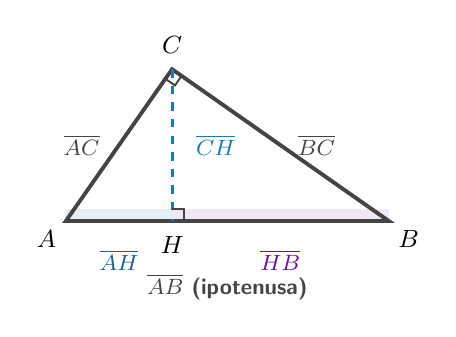
\begin{tikzpicture}[x=0.82cm, y=0.82cm]
  \coordinate (A) at (0,0);
  \coordinate (B) at (5,0);
  \coordinate (C) at (1.645,2.350);
  \coordinate (H) at (1.645,0);

  % Sfondo proiezioni
  \fill[azzurro!12] (A) rectangle ($(H)+(0,0.18)$);
  \fill[tpurple!10] (H) rectangle ($(B)+(0,0.18)$);

  % Lati del triangolo
  \draw[dark, line width=1.4pt] (A) -- (B) -- (C) -- cycle;

  % Altezza CH tratteggiata
  \draw[azzurro, line width=1.1pt, dashed] (C) -- (H);

  % Quadratino angolo retto in C
  \coordinate (qCA) at ($(C)+0.18*(-0.576,-0.822)$);
  \coordinate (qCB) at ($(C)+0.18*(0.820,-0.574)$);
  \coordinate (qCC) at ($(C)+0.18*(-0.576,-0.822)+0.18*(0.820,-0.574)$);
  \draw[dark, line width=0.7pt] (qCA) -- (qCC) -- (qCB);

  % Quadratino angolo retto in H
  \draw[dark, line width=0.7pt]
    ($(H)+(0.18,0)$) -- ($(H)+(0.18,0.18)$) -- ($(H)+(0,0.18)$);

  % Etichette vertici
  \node[below left,  font=\small\bfseries] at (A) {$A$};
  \node[below right, font=\small\bfseries] at (B) {$B$};
  \node[above, font=\small\bfseries, yshift=2pt] at (C) {$C$};
  \node[below, font=\small\bfseries, yshift=-2pt] at (H) {$H$};

  % Etichette segmenti
  \node[below, font=\footnotesize, color=azzurro!80!black]
    at ($(A)!0.5!(H)+(0,-0.30)$) {$\overline{AH}$};
  \node[below, font=\footnotesize, color=tpurple]
    at ($(H)!0.5!(B)+(0,-0.30)$) {$\overline{HB}$};
  \node[left,  font=\footnotesize, color=dark]
    at ($(A)!0.5!(C)+(-0.15,0)$) {$\overline{AC}$};
  \node[right, font=\footnotesize, color=dark]
    at ($(B)!0.5!(C)+(0.12,0)$)  {$\overline{BC}$};
  \node[right, font=\footnotesize, color=azzurro]
    at ($(C)!0.5!(H)+(0.22,0)$)  {$\overline{CH}$};
  \node[below, font=\footnotesize\bfseries, color=dark, yshift=-0.55cm]
    at ($(A)!0.5!(B)$) {$\overline{AB}$ (ipotenusa)};
\end{tikzpicture}
\end{center}

{\footnotesize\color{mgray}
L'angolo retto $\hat{C}$ è in $C$; $H$ è il \emph{piede}
dell'altezza $CH \perp AB$. Il simbolo $\square$ indica 90°.}
\bigskip

%%──────────────────────────────────────────────────────────
\sectitle{Esercizi — Primo Teorema di Euclide}

{\footnotesize\color{mgray}\textit{Calcola il perimetro
applicando il primo teorema di Euclide.}}
\bigskip

\enum
\begin{eserciziobox}
\textbf{a)} $\overline{AH}=9$ cm, $\overline{AC}=216$ cm. Calcola il perimetro.\\
\textbf{b)} Ipotenusa $=225$ cm, proiezione $=221$ cm. Calcola il perimetro.
\end{eserciziobox}

\enum
\begin{eserciziobox}
\textbf{a)} $\overline{AC}=64$ cm, $\overline{AH}=40$ cm. Calcola il perimetro.\\
\textbf{b)} $\overline{BC}=25$ cm, $\overline{BH}=16$ cm. Calcola il perimetro.
\end{eserciziobox}

\enum
\begin{eserciziobox}
\textbf{a)} $\overline{AH}=18$ cm, $\overline{HB}=32$ cm. Calcola il perimetro.
\begin{solbox}
$\overline{AB}=50$ cm;\;
$\overline{AC}^2=50\!\cdot\!18=900$ $cm^2\Rightarrow\overline{AC}=30$ cm;\;
$\overline{BC}^2=50\!\cdot\!32=1600$ $cm^2 \Rightarrow\overline{BC}=40$ cm.\\
$2p = 50+30+40 = \mathbf{120}$ cm.
\end{solbox}
\textbf{b)} Altezza $\overline{CH}=75$ cm, $\hat{B}=45^\circ$.\\
\textbf{c)} $\overline{AH}=4{,}5$ cm, $\overline{HB}=12{,}5$ cm.
\end{eserciziobox}


\enum
\begin{eserciziobox}
Triangolo isoscele $ABC$: lato $=16$ cm, altezza $=12{,}8$ cm.
Determina il raggio della circonferenza circoscritta.%
\risultato{10\text{ cm}}
\end{eserciziobox}

%%══════════════════════════════════════════════════════════
%%  02  PROBLEMI CON EQUAZIONI — EUCLIDE
%%══════════════════════════════════════════════════════════
\seclabel{02 · Problemi con equazioni — Euclide}

\enumsv{Completamento dello svolgimento}
\begin{fondamentali}
La proiezione di un cateto sull'ipotenusa è $\tfrac{4}{9}$ del
cateto stesso; l'altra proiezione è 65 cm.
Determina il perimetro del triangolo.
\end{fondamentali}

\noindent\textit{Svolgimento.}
Sia $\overline{AC}=x$, allora $\overline{AH}=\tfrac{4}{9}x$.
\[
x^2=\tfrac{4}{9}x\!\left(\tfrac{4}{9}x+65\right)
\;\Rightarrow\; x^2-36x=0 \;\Rightarrow\; x=36.
\]
Quindi $\overline{AC}=36$, $\overline{AH}=16$, $\overline{AB}=81$.
\[
\overline{BC}=\sqrt{65\cdot81}=9\sqrt{65}.
\quad
\boxed{2p = 117+9\sqrt{65}\ \text{cm.}}
\]

\enum
\begin{eserciziobox}
Cateto $=60$ cm, proiezione $=36$ cm. Calcola il perimetro.%
\risultato{240\text{ cm}}
\end{eserciziobox}

\enum
\begin{eserciziobox}
Cateto $=165$ cm, ipotenusa $=275$ cm. Determina l'altezza
relativa all'ipotenusa.\risultato{132\text{ cm}}
\end{eserciziobox}

\enum
\begin{eserciziobox}
Cateti $4x$ e $9x$; altezza relativa all'ipotenusa $=18$ cm.
Calcola l'area.\risultato{108\text{ cm}^2}
\end{eserciziobox}

\enum
\begin{eserciziobox}
Ipotenusa $=50$ cm; un cateto $=\tfrac{5}{4}$ della sua proiezione.
Calcola il perimetro.\risultato{120\text{ cm}}
\end{eserciziobox}

\enum
\begin{eserciziobox}
Cateti $60$ cm e $80$ cm. Determina le due proiezioni
sull'ipotenusa.\risultato{36;\;64\text{ cm}}
\end{eserciziobox}

\enum
\begin{eserciziobox}
Il cateto maggiore è $\tfrac{5}{4}$ della sua proiezione ed è
il doppio dell'altra proiezione $+2a$.
Determina l'area.\risultato{150a^2}
\end{eserciziobox}

\enum
\begin{eserciziobox}
La proiezione maggiore supera il cateto minore di 9 cm; il
cateto minore è $\tfrac{3}{5}$ dell'ipotenusa.
Determina l'area.\risultato{12150\text{ cm}^2}
\end{eserciziobox}

%%══════════════════════════════════════════════════════════
%%  03  TEOREMA DI PITAGORA
%%══════════════════════════════════════════════════════════
\seclabel{03 · Teorema di Pitagora}

\begin{defbox}[tpurple]{Enunciato}
In un triangolo rettangolo il \textbf{quadrato sull'ipotenusa}
è equivalente alla \textbf{somma dei quadrati sui cateti}.
\end{defbox}

\begin{formula}
$c^{2} = a^{2} + b^{2}$
\end{formula}

\sectitle{Figura di riferimento}

% ── Note sui calcoli ────────────────────────────────────
% A=(0,0), B=(3,0), C=(3,2.25) — angolo retto in B
% Quadrato su AB (a=3): vertici (0,0),(3,0),(3,-3),(0,-3)
% Quadrato su BC (b=2.25): vertici (3,0),(3,2.25),(5.25,2.25),(5.25,0)
% Quadrato su AC (c=3.75, ipotenusa):
%   perp. unit. di AC = (-2.25,3)/3.75 = (-0.6, 0.8)
%   D = A + 3.75*(-0.6,0.8) = (-2.25, 3.0)
%   E = C + 3.75*(-0.6,0.8) = (0.75, 5.25)
% ────────────────────────────────────────────────────────

\begin{center}
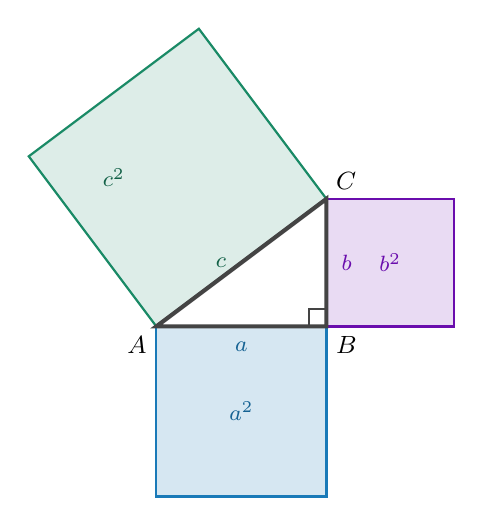
\begin{tikzpicture}[x=0.72cm, y=0.72cm]
  \coordinate (A) at (0,0);
  \coordinate (B) at (3,0);
  \coordinate (C) at (3,2.25);
  \coordinate (D) at (-2.25,3.0);
  \coordinate (E) at (0.75,5.25);

  % Quadrato su AB — sotto
  \fill[azzurro!18] (A)--(B)--(3,-3)--(0,-3)--cycle;
  \draw[azzurro, line width=0.8pt] (A)--(B)--(3,-3)--(0,-3)--cycle;
  \node[font=\footnotesize\bfseries, color=azzurro!80!black] at (1.5,-1.5) {$a^2$};

  % Quadrato su BC — destra
  \fill[tpurple!15] (B)--(C)--(5.25,2.25)--(5.25,0)--cycle;
  \draw[tpurple, line width=0.8pt] (B)--(C)--(5.25,2.25)--(5.25,0)--cycle;
  \node[font=\footnotesize\bfseries, color=tpurple] at (4.125,1.125) {$b^2$};

  % Quadrato su AC — ipotenusa, sinistra
  \fill[tgreen!15] (A)--(C)--(E)--(D)--cycle;
  \draw[tgreen, line width=0.8pt] (A)--(C)--(E)--(D)--cycle;
  \node[font=\footnotesize\bfseries, color=tgreen!70!black] at (-0.75,2.625) {$c^2$};

  % Triangolo (sopra tutto)
  \draw[dark, line width=1.5pt] (A)--(B)--(C)--cycle;

  % Angolo retto in B
  \draw[dark, line width=0.7pt] (2.7,0)--(2.7,0.3)--(3,0.3);

  % Etichette vertici
  \node[below left,  font=\small\bfseries] at (A) {$A$};
  \node[below right, font=\small\bfseries] at (B) {$B$};
  \node[above right, font=\small\bfseries] at (C) {$C$};

  % Etichette lati
  \node[below, font=\footnotesize, color=azzurro!80!black, yshift=-2pt]
    at ($(A)!0.5!(B)$) {$a$};
  \node[right, font=\footnotesize, color=tpurple, xshift=2pt]
    at ($(B)!0.5!(C)$) {$b$};
  \node[left,  font=\footnotesize, color=tgreen!70!black, xshift=-2pt]
    at ($(A)!0.5!(C)$) {$c$};
\end{tikzpicture}
\end{center}

{\footnotesize\color{mgray}
$a,b$: cateti; $c$: ipotenusa; angolo retto in $B$.}
\vspace{4pt}

%%──────────────────────────────────────────────────────────
\sectitle{Esercizi — Teorema di Pitagora}

\enum
\begin{eserciziobox}
In $\triangle DAB$: $DA=5$, $DC=13$, $CB=7$, $DH\perp AB$.
Trova: 1)~$\overline{AB}$;\; 2)~$\overline{CD}$;\;
3)~$\overline{CH}$;\; 4)~$\overline{HB}$.\\
\textit{Ris.:} 12;\;$\sqrt{218}$;\;5;\;$2\sqrt{6}$
\end{eserciziobox}

\enum
\begin{eserciziobox}
Cateto $=48$ cm, area $=336$ cm$^2$. Ipotenusa?%
\risultato{50\text{ cm}}
\end{eserciziobox}

\enum
\begin{eserciziobox}
Lato del quadrato $\cong$ diagonale del rettangolo $12\times5$ cm.
Area e perimetro del quadrato.%
\risultato{169\text{ cm}^2;\;52\text{ cm}}
\end{eserciziobox}

\enum
\begin{eserciziobox}
Rombo: diagonale maggiore $48a$, minore $=\tfrac{5}{12}$ della
maggiore. Perimetro.\risultato{104a}
\end{eserciziobox}

\enuml{INVALSI}
\begin{eserciziobox}
Scala da 5 gradini ($24\times18$ cm). Lunghezza dello scivolo?
\begin{enumerate}[label=\Alph*),noitemsep,topsep=2pt,leftmargin=*]
  \item $(\sqrt{18^2+24^2})\cdot5$
  \item $\sqrt{(24+18)^2\cdot5}$
  \item $\sqrt{24^2+18^2}\cdot5\quad\textcolor{tgreen}{\checkmark}$
  \item $\sqrt{(24^3+18^2)\cdot5}$
\end{enumerate}
\end{eserciziobox}

\enuml{Intorno a noi}
\begin{eserciziobox}
Pendenza 10\% (10 m ogni 100 m). Spostamento orizzontale 4725 m:
dislivello e strada percorsa.%
\risultato{472{,}5\text{ m};\;\approx4748{,}6\text{ m}}
\end{eserciziobox}

\enuml{INVALSI — Tavoletta babilonese (1800 a.C.)}
\begin{eserciziobox}
Bastone di 10 unità appoggiato al muro; scivola di 2 unità verso
il basso. Di quante unità si allontana il piede dalla base?\\
\textbf{A}~6\quad\textbf{B}~8\quad\textbf{C}~10\quad\textbf{D}~12
\end{eserciziobox}

%%══════════════════════════════════════════════════════════
%%  04  PROBLEMI CON EQUAZIONI — PITAGORA
%%══════════════════════════════════════════════════════════
\seclabel{04 · Problemi con equazioni — Pitagora}

\enumsv{Completamento dello svolgimento}
\begin{fondamentali}
Cateti $\tfrac{1}{2}x$ e $(x-2)$ con $x>2$; ipotenusa $=34$ cm.
Determina i cateti.
\end{fondamentali}

\noindent\textit{Svolgimento.}
$\bigl(\tfrac{x}{2}\bigr)^2+(x-2)^2=34^2
\Rightarrow 5x^2-16x-4608=0.$
\[
x_1=-\tfrac{144}{5}\ (\text{scartata}),\quad x_2=32.
\]
\[
\overline{AC}=30\text{ cm},\quad\overline{AB}=16\text{ cm}.
\]

\enumsv{Completamento dello svolgimento}
\begin{fondamentali}
Un cateto è $\tfrac{5}{12}$ dell'altro; perimetro $=180$ cm.
Trova i tre lati.
\end{fondamentali}

\noindent\textit{Svolgimento.}
Sia $\overline{AC}=x$, $\overline{AB}=\tfrac{5}{12}x$,
$\overline{BC}=\tfrac{13}{12}x$.
\[
x+\tfrac{5}{12}x+\tfrac{13}{12}x=180\;\Rightarrow\;x=72.
\]
\[
\overline{AC}=72,\;\overline{AB}=30,\;\overline{BC}=78\text{ cm}.
\]

\enum
\begin{eserciziobox}
Triangolo isoscele: base $=\tfrac{5}{2}$ lato, altezza $=3$ cm.
Calcola l'area.\risultato{\text{nessuna soluzione}}
\end{eserciziobox}

\enum
\begin{eserciziobox}
Area $=600$ cm$^2$; un cateto $=\tfrac{4}{5}$ ipotenusa. Cateti.%
\risultato{40;\;30\text{ cm}}
\end{eserciziobox}

\enum
\begin{eserciziobox}
Rombo, area $=216$ cm$^2$, diagonale maggiore $=\tfrac{8}{5}$
del lato. Perimetro.\risultato{60\text{ cm}}
\end{eserciziobox}

\enum
\begin{eserciziobox}
Perimetro $=40$ cm; ipotenusa $=$ somma cateti $-6$. Cateti.%
\risultato{15;\;8\text{ cm}}
\end{eserciziobox}

%%══════════════════════════════════════════════════════════
%%  05  APPLICAZIONI — DIAGONALE E ALTEZZA EQUILATERO
%%══════════════════════════════════════════════════════════
\seclabel{05 · Applicazioni del Teorema di Pitagora}

\begin{formulag}
Diagonale del quadrato di lato $\ell$:\quad $d=\ell\sqrt{2}$
\end{formulag}

\begin{formulao}
Altezza del triangolo equilatero di lato $\ell$:\quad
$h=\dfrac{\ell\sqrt{3}}{2}$
\end{formulao}

\enuml{TEST}
\begin{eserciziobox}
Diagonale di un quadrato di lato 7 cm?\\
\textbf{A}~$7\sqrt{2}$\quad
\textbf{B}~14\quad
\textbf{C}~$\dfrac{7}{\sqrt{2}}$\quad
\textbf{D}~28 cm
\end{eserciziobox}

\enum
\begin{eserciziobox}
Le mezze-diagonali misurano $5\sqrt{2}$ cm. Area e perimetro
del quadrato.\risultato{100\text{ cm}^2;\;40\text{ cm}}
\end{eserciziobox}

\enuml{Sport}
\begin{eserciziobox}
Casa base--centro diamante $=19$ m. Perimetro e area.%
\risultato{76\sqrt{2}\text{ m};\;722\text{ m}^2}
\end{eserciziobox}

\enuml{TEST}
\begin{eserciziobox}
Altezza triangolo equilatero $=10$ cm. Lato?\\
\textbf{A}~$10\sqrt{3}$\quad
\textbf{B}~$\dfrac{10\sqrt{3}}{3}$\quad
\textbf{C}~$\dfrac{20\sqrt{3}}{3}$\quad
\textbf{D}~10 cm
\end{eserciziobox}

\enum
\begin{eserciziobox}
Raggi della circoscritta e inscritta a un triangolo equilatero
di lato 3.\risultato{\dfrac{\sqrt{3}}{2};\;\sqrt{3}}
\end{eserciziobox}

\enuml{INVALSI}
\begin{eserciziobox}
Triangolo equilatero e quadrato con ugual perimetro; area
triangolo $=9\sqrt{3}$ cm$^2$. Lato del quadrato?\\
\textbf{A}~$2\sqrt{3}$\quad
\textbf{B}~$\dfrac{9}{2}$\quad
\textbf{C}~$\dfrac{9\sqrt{2}}{2}$\quad
\textbf{D}~8
\end{eserciziobox}

\enum
\begin{eserciziobox}
$\hat{A}=45°$, $\hat{C}=60°$, $BC=12$ cm. Perimetro e area.%
\risultato{6(3{+}\sqrt{3}{+}\sqrt{6});\;18(3{+}\sqrt{3})\text{ cm}^2}
\end{eserciziobox}

%%══════════════════════════════════════════════════════════
%%  06  SECONDO TEOREMA DI EUCLIDE
%%══════════════════════════════════════════════════════════
\seclabel{06 · Secondo Teorema di Euclide}

\begin{defbox}[azzurro]{Enunciato}
Il \textbf{quadrato sull'altezza} relativa all'ipotenusa è
equivalente al \textbf{rettangolo avente per lati le proiezioni}
dei cateti sull'ipotenusa.
\end{defbox}

\begin{formula}
$\overline{CH}^{2} = \overline{AH}\cdot\overline{BH}$
\end{formula}

\sectitle{Esempio — Calcolo senza Pitagora}

\begin{fondamentali}
Dati: $\overline{CM}=30{,}5$ cm (mediana $\Rightarrow$
$\overline{AB}=61$ cm), $\overline{HB}=100$ cm.\\
$\overline{AH}=116-100=16$.\quad
$2°$~teo.: $\overline{CH}^2=16\cdot100\Rightarrow\overline{CH}=40$.\\
$1°$~teo.:
$\overline{AC}=\sqrt{116\cdot16}=8\sqrt{29}$,\;
$\overline{BC}=\sqrt{116\cdot100}=20\sqrt{29}$.\\
$2p(ABC)=4(7\sqrt{29}+29)$;\;
$2p(BCH)=20(7+\sqrt{29})$.
\end{fondamentali}

\sectitle{Esercizi — Secondo Teorema di Euclide}

\enuml{TEST}
\begin{eserciziobox}
Cateti 12 e 3. Misura di $\overline{AH}$?\\
\textbf{A}~$\sqrt{45}$\quad
\textbf{B}~36\quad
\textbf{C}~6\quad
\textbf{D}~15
\end{eserciziobox}

\enum
\begin{eserciziobox}
Altezza $=12$ m, proiezione $=18$ m. Perimetro e area.%
\risultato{(26{+}10\sqrt{13})\text{ m};\;156\text{ m}^2}
\end{eserciziobox}

\enum
\begin{eserciziobox}
Trapezio $ABCD$: $BD\perp AD$; base maggiore $=20$ cm,
proiezione $AD=4$ cm. Area.\risultato{112\text{ cm}^2}
\end{eserciziobox}

\enum
\begin{eserciziobox}
Rombo: perimetro $=40$ cm, diag.\ minore $=12$ cm.
Area; $AL$, $LB$, $OL$.%
\risultato{96\text{ cm}^2;\;3{,}6;\;6{,}4;\;4{,}8\text{ cm}}
\end{eserciziobox}

%%══════════════════════════════════════════════════════════
%%  07  PROBLEMI CON EQUAZIONI — SECONDO TEOREMA
%%══════════════════════════════════════════════════════════
\seclabel{07 · Problemi con equazioni — II Teorema}

\enumsv{Completamento dello svolgimento}
\begin{fondamentali}
Mediana $\overline{CM}=30{,}5$ cm;
$\overline{CH}=\tfrac{60}{11}\,\overline{HM}$.
Perimetro di $HMC$.
\end{fondamentali}

\noindent\textit{Svolgimento.}
$\overline{AB}=61$;\;
$\overline{HM}=x$;\;$\overline{CH}=\tfrac{60}{11}x$.
\[
\!\left(\tfrac{60}{11}x\right)^{\!2}=
\left(\tfrac{61}{2}-x\right)\!\left(\tfrac{61}{2}+x\right)
\;\Rightarrow\;x=\tfrac{11}{2}.
\]
\[
\overline{CH}=30;\quad
2p(HMC)=\tfrac{61}{2}+\tfrac{11}{2}+30=66\text{ cm}.
\]

\enum
\begin{eserciziobox}
Area $=980$ cm$^2$; una proiezione $=\tfrac{1}{4}$ dell'altra.
Ipotenusa.\risultato{70\text{ cm}}
\end{eserciziobox}

\enum
\begin{eserciziobox}
Trapezio isoscele: base minore $=5{,}6$ m,
proiezione lato $=7{,}2$ m, diag.\ $\perp$ lato obliquo.
Perimetro e area.%
\risultato{49{,}6\text{ m};\;122{,}88\text{ m}^2}
\end{eserciziobox}

%%══════════════════════════════════════════════════════════
%%  08  FAI IL PUNTO SULLE COMPETENZE
%%══════════════════════════════════════════════════════════
\seclabel{08 · Fai il punto sulle competenze}

\enuml{Vero o Falso?}
\begin{eserciziobox}
$ED\!\parallel\!AB$, $PR\!\parallel\!QD$. V o F?
\begin{enumerate}[label=\alph*),noitemsep,topsep=1pt,leftmargin=*]
  \item $\overline{BE}^2=\overline{BP}\cdot\sqrt{\overline{AE}^2+\overline{BE}^2}$
  \item $\overline{PR}^2=\overline{ER}\cdot\overline{EB}-\overline{ER}^2$
  \item $\overline{BD}^2-\overline{EB}^2=\overline{EQ}\cdot\overline{EB}$
  \item $\overline{ED}^2=\overline{BR}^2+\overline{PR}^2$
\end{enumerate}
\end{eserciziobox}

\enuml{INVALSI}
\begin{eserciziobox}
Scatola $6\times6\times3$ cm. Lunghezza max dello stecchino?\\
\textbf{A}~6\quad\textbf{B}~7\quad\textbf{C}~8\quad
\textbf{D}~9\quad\textbf{E}~10 cm
\end{eserciziobox}

\enum
\begin{eserciziobox}
Rettangolo $ABCD$: $AB=4$, $BC=2$ cm. Trova $P$ su $AB$ tale che
$\overline{PA}^2+\overline{PB}^2+\overline{PC}^2+\overline{PD}^2=33$.
\end{eserciziobox}

\enum
\begin{eserciziobox}
Triangolo isoscele: lato $=\tfrac{3}{5}\sqrt{10}\,a$,
altezza alla base $=\tfrac{3}{2}$ della base. Perimetro.
\end{eserciziobox}

\enum
\begin{eserciziobox}
Trapezio rettangolo: diag.\ minore $\perp$ lato obliquo;
altezza $=\tfrac{3}{4}$ base minore; lato obl.\ $=3a$.
Area e perimetro.
\end{eserciziobox}

\enum
\begin{eserciziobox}
Trapezio scaleno: angoli alla base maggiore 30° e 45°;
base minore $=$ altezza $=10$ m. Perimetro e area.
\end{eserciziobox}

%%══════════════════════════════════════════════════════════
%%  09  TRIANGOLI INSCRITTI NELLA CIRCONFERENZA
%%      E APPLICAZIONI DEI TEOREMI DI EUCLIDE
%%══════════════════════════════════════════════════════════
\seclabel{09 · Triangoli inscritti e Teoremi di Euclide}

% ── Teorema dell'angolo inscrito ─────────────────────────
\begin{defbox}[tpurple]{Angolo inscrito su diametro}
Ogni triangolo inscritto in una semicirconferenza ha
l'\textbf{angolo opposto al diametro retto} ($= 90°$).\\[2pt]
Se $AB$ è diametro e $C$ è un punto della circonferenza,
allora $\hat{C}=90°$.
\end{defbox}

\sectitle{Figura di riferimento — triangolo in semicirconferenza}

% Triangolo rettangolo inscritto:
%   O=(0,0), r=2.5, A=(-2.5,0), B=(2.5,0) diametro
%   C = 2.5*(cos70°, sin70°) = (0.855, 2.349)
%   angolo retto in C (Talete)
%   H = piede altezza da C su AB = (0.855, 0)
%   Mediana CM: M=midpoint(AB)=(0,0)=O => CM=r=2.5
%   Proiezioni: AH=2.5+0.855=3.355, HB=2.5-0.855=1.645

\begin{center}
% ── Coordinate (tutte in cm, nessuna scala personalizzata) ──
% O=(0,0), r=2.2cm
% A=(-2.2,0), B=(2.2,0)  [estremi del diametro]
% C sulla semicirconferenza a 70° da B:
%   C = (2.2*cos70°, 2.2*sin70°) = (0.753, 2.067)
%   angolo retto in C garantito da Talete
% H = piede altezza = (0.753, 0)
% Quadratino in C:
%   CA=(-2.2-0.753, -2.067)=(-2.953,-2.067), |CA|=3.606
%     unitCA=(-0.819,-0.573)
%   CB=(2.2-0.753,-2.067)=(1.447,-2.067), |CB|=2.527
%     unitCB=(0.572,-0.818)
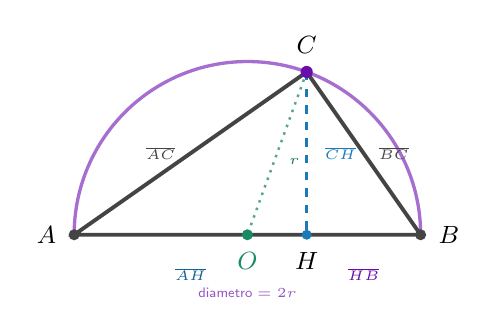
\begin{tikzpicture}
  \coordinate (O) at (0,0);
  \coordinate (A) at (-2.2cm,0);
  \coordinate (B) at ( 2.2cm,0);
  \coordinate (C) at (0.753cm,2.067cm);
  \coordinate (H) at (0.753cm,0);

  % Semicirconferenza — arc centrato in O, raggio 2.2cm
  \draw[tpurple!60, line width=1.2pt]
        (A) arc[start angle=180, end angle=0, radius=2.2cm];

  % Diametro AB (tratto grigio sotto il triangolo)
  \draw[dark!35, line width=0.7pt] (A) -- (B);

  % Triangolo
  \draw[dark, line width=1.4pt] (A) -- (B) -- (C) -- cycle;

  % Altezza CH tratteggiata
  \draw[azzurro, line width=1pt, dashed] (C) -- (H);

  % Mediana CO = raggio (punteggiata verde)
  \draw[tgreen!75, line width=0.9pt, dotted] (C) -- (O);

  % Punti
  \fill[dark]    (A) circle(2pt);
  \fill[dark]    (B) circle(2pt);
  \fill[tpurple] (C) circle(2.2pt);
  \fill[azzurro] (H) circle(1.8pt);
  \fill[tgreen]  (O) circle(2pt);

  % Etichette vertici
  \node[left,  font=\small\bfseries, xshift=-3pt] at (A) {$A$};
  \node[right, font=\small\bfseries, xshift=3pt]  at (B) {$B$};
  \node[above, font=\small\bfseries, yshift=3pt]  at (C) {$C$};
  \node[below, font=\small\bfseries, yshift=-3pt] at (H) {$H$};
  \node[below, font=\small\bfseries, color=tgreen, yshift=-3pt] at (O) {$O$};

  % Etichette segmenti
  \node[below, font=\tiny, color=azzurro!80!black]
    at ($(A)!0.5!(H)+(0,-0.3cm)$) {$\overline{AH}$};
  \node[below, font=\tiny, color=tpurple]
    at ($(H)!0.5!(B)+(0,-0.3cm)$) {$\overline{HB}$};
  \node[left,  font=\tiny, color=dark, xshift=-2pt]
    at ($(A)!0.5!(C)$) {$\overline{AC}$};
  \node[right, font=\tiny, color=dark, xshift=2pt]
    at ($(B)!0.5!(C)$) {$\overline{BC}$};
  \node[right, font=\tiny, color=azzurro, xshift=3pt]
    at ($(C)!0.5!(H)$) {$\overline{CH}$};
  \node[right, font=\tiny, color=tgreen!80!black, xshift=2pt]
    at ($(C)!0.55!(O)$) {$r$};

  % Etichetta diametro
  \node[below, font=\tiny, color=tpurple!70, yshift=-0.55cm]
    at ($(A)!0.5!(B)$) {diametro $= 2r$};
\end{tikzpicture}
\end{center}

{\footnotesize\color{mgray}
$O$ = centro; $r$ = raggio; $AB$ = diametro; $\hat{C}=90°$
(teorema di Talete). La mediana $\overline{CO}=r$.}
\vspace{4pt}

% ── Proprietà chiave ─────────────────────────────────────
\begin{defbox}[tgreen]{Proprietà fondamentali}
Nel triangolo rettangolo $ABC$ inscritto di diametro $AB=2r$:
\begin{enumerate}[noitemsep,topsep=2pt,leftmargin=*]
  \item $\hat{C}=90°$ \textbf{(teorema di Talete)}
  \item La mediana relativa all'ipotenusa
        $\overline{CO}=r=\tfrac{\overline{AB}}{2}$
  \item $1°$ Euclide:\;
        $\overline{AC}^2=\overline{AB}\cdot\overline{AH}$,\;
        $\overline{BC}^2=\overline{AB}\cdot\overline{BH}$
  \item $2°$ Euclide:\;
        $\overline{CH}^2=\overline{AH}\cdot\overline{BH}$
  \item $\overline{CH}=\dfrac{\overline{AC}\cdot\overline{BC}}{\overline{AB}}$
        \quad (altezza sul diametro)
\end{enumerate}
\end{defbox}

\sectitle{Esempio svolto}

\begin{fondamentali}
\textbf{Problema.} Un triangolo rettangolo è inscritto in una
circonferenza di raggio $r=5$ cm. Uno dei cateti misura 6 cm.
Determina l'altro cateto, l'altezza sull'ipotenusa e le due
proiezioni dei cateti.

\medskip
\textbf{Soluzione.}
$\overline{AB}=2r=10$ cm (ipotenusa = diametro).

Pitagora: $\overline{BC}=\sqrt{10^2-6^2}=\sqrt{64}=8$ cm.

$1°$ Euclide:
\[
\overline{AH}=\frac{\overline{AC}^2}{\overline{AB}}
             =\frac{36}{10}=3{,}6\text{ cm};\quad
\overline{BH}=\frac{\overline{BC}^2}{\overline{AB}}
             =\frac{64}{10}=6{,}4\text{ cm}.
\]
$2°$ Euclide:
\[
\overline{CH}=\sqrt{\overline{AH}\cdot\overline{BH}}
             =\sqrt{3{,}6\cdot6{,}4}=\sqrt{23{,}04}=4{,}8\text{ cm}.
\]
Verifica: $\overline{CH}=\tfrac{6\cdot8}{10}=4{,}8$ cm.\;\checkmark
\end{fondamentali}

\sectitle{Esercizi — Triangoli inscritti}

\enum
\begin{eserciziobox}
Un triangolo rettangolo è inscritto in una circonferenza di
raggio 13 cm. Un cateto misura 10 cm. Calcola l'altro cateto,
l'altezza sull'ipotenusa e le due proiezioni dei cateti.%
\risultato{\overline{BC}\approx17{,}3;\;\overline{CH}\approx8{,}3\text{ cm}}
\end{eserciziobox}

\enum
\begin{eserciziobox}
Un triangolo isoscele rettangolo è inscritto in una
circonferenza di raggio $r$. Calcola il lato e l'area
in funzione di $r$.\risultato{\ell=r\sqrt{2};\;A=r^2}
\end{eserciziobox}

\enum
\begin{eserciziobox}
Un triangolo rettangolo inscritto ha ipotenusa $=26$ cm e
un cateto $=24$ cm. Calcola il raggio della circonferenza
circoscritta, le due proiezioni sull'ipotenusa e l'altezza.%
\risultato{r=13;\;\overline{AH}=\tfrac{144}{13};\;
\overline{BH}=\tfrac{100}{13};\;\overline{CH}=\tfrac{120}{13}\text{ cm}}
\end{eserciziobox}

\enum
\begin{eserciziobox}
In una circonferenza di raggio 10 cm è inscritto un triangolo
rettangolo con proiezioni dei cateti in rapporto $1:4$.
Calcola i cateti e l'altezza sull'ipotenusa.%
\risultato{\overline{AC}=4\sqrt{5};\;\overline{BC}=8\sqrt{5};\;
\overline{CH}=8\text{ cm}}
\end{eserciziobox}

\enum
\begin{eserciziobox}
L'altezza relativa all'ipotenusa di un triangolo rettangolo
inscritto in una circonferenza di raggio 7{,}5 cm è lunga 9 cm.
Calcola i due cateti e le due proiezioni.%
\risultato{\overline{AC}=12;\;\overline{BC}=9;\;
\overline{AH}=9{,}6;\;\overline{BH}=5{,}4\text{ cm}}
\end{eserciziobox}

\enum
\begin{eserciziobox}
Un triangolo rettangolo inscritto in una semicirconferenza ha
la proiezione del cateto maggiore sull'ipotenusa uguale a
$\tfrac{3}{4}$ dell'ipotenusa. Il cateto minore misura 6 cm.
Calcola il raggio della circonferenza circoscritta.%
\risultato{r=\tfrac{\sqrt{3}}{2}\cdot4\sqrt{3}=6\text{ cm}}
\end{eserciziobox}

\enumsv{Completamento dello svolgimento}
\begin{fondamentali}
Un triangolo rettangolo $ABC$ è inscritto in una circonferenza
di centro $O$ e raggio $r$. La mediana $\overline{CM}=10$ cm
e la proiezione $\overline{AH}=8$ cm.
Calcola il raggio, i cateti e l'altezza sull'ipotenusa.
\end{fondamentali}

\noindent\textit{Svolgimento.}
Poiché la mediana relativa all'ipotenusa è metà dell'ipotenusa:
\[
r = \overline{CM} = 10\text{ cm},\quad
\overline{AB}=2r=20\text{ cm},\quad
\overline{BH}=20-8=12\text{ cm}.
\]
$1°$ Euclide:
\[
\overline{AC}=\sqrt{20\cdot8}=\sqrt{160}=4\sqrt{10}\text{ cm},\quad
\overline{BC}=\sqrt{20\cdot12}=\sqrt{240}=4\sqrt{15}\text{ cm}.
\]
$2°$ Euclide:
\[
\overline{CH}=\sqrt{8\cdot12}=\sqrt{96}=4\sqrt{6}\text{ cm}.
\]

\enum
\begin{eserciziobox}
Un triangolo rettangolo inscritto ha diametro $=30$ cm e
proiezione $\overline{AH}=9$ cm. Calcola cateti, altezza
sull'ipotenusa e perimetro.\risultato{\overline{AC}=\!9\sqrt{10};\;
\overline{BC}=\!3\sqrt{70};\;\overline{CH}=\!9\sqrt{7}\text{ cm}}
\end{eserciziobox}

\enum
\begin{eserciziobox}
In un triangolo rettangolo inscritto in una circonferenza di
raggio 6{,}5 cm, i cateti sono in rapporto $5:12$.
Calcola: cateti, altezza sull'ipotenusa, proiezioni e area.%
\risultato{5;\;12;\;h=\tfrac{60}{13};\;p_1=\tfrac{25}{13};\;
p_2=\tfrac{144}{13};\;A=30\text{ cm}^2}
\end{eserciziobox}

\enum
\begin{eserciziobox}
Un triangolo equilatero di lato $\ell$ è inscritto in una
circonferenza. Usando il teorema di Pitagora, dimostra che
il raggio della circoscritta è $R=\dfrac{\ell\sqrt{3}}{3}$
e quello dell'inscritta è $r=\dfrac{\ell\sqrt{3}}{6}$.
\end{eserciziobox}

\enum
\begin{eserciziobox}
Un poligono regolare di 6 lati (esagono) è inscritto in una
circonferenza di raggio $r=8$ cm. Calcola il lato, il perimetro
e l'apotema dell'esagono, applicando il teorema di Pitagora.%
\risultato{\ell=8;\;2p=48;\;a=4\sqrt{3}\text{ cm}}
\end{eserciziobox}

\enum
\begin{eserciziobox}
Un quadrato è inscritto in una circonferenza di raggio $r$.
Calcola il lato, la diagonale, il perimetro e l'area del
quadrato in funzione di $r$.%
\risultato{\ell=r\sqrt{2};\;d=2r;\;P=4r\sqrt{2};\;A=2r^2}
\end{eserciziobox}

%%──────────────────────────────────────────────────────────
\sectitle{Applicazioni dei Teoremi di Euclide}
%%──────────────────────────────────────────────────────────

\begin{defbox}[orange]{Schema risolutivo}
Per un triangolo rettangolo $ABC$ con $\hat{C}=90°$,
altezza $CH$ e proiezioni $\overline{AH}$, $\overline{HB}$:
\[
\overline{AC}^2=\overline{AB}\cdot\overline{AH},\quad
\overline{BC}^2=\overline{AB}\cdot\overline{BH},\quad
\overline{CH}^2=\overline{AH}\cdot\overline{BH}.
\]
Se il triangolo è \textbf{inscritto nel cerchio}:
$\overline{AB}=2r$ e $\overline{CO}=r$.
\end{defbox}

\enum
\begin{eserciziobox}
Corda e secante. In una circonferenza di raggio 10 cm,
una corda $\overline{AB}=16$ cm. Calcola la distanza della
corda dal centro e le due parti in cui il diametro
perpendicolare alla corda divide quest'ultima.%
\risultato{d=6;\;\overline{AM}=\overline{MB}=8\text{ cm}}
\end{eserciziobox}

\enum
\begin{eserciziobox}
Altezza sul diametro. Un punto $C$ sulla circonferenza di
raggio 15 cm proietta sul diametro $AB$ in $H$, con
$\overline{AH}=9$ cm. Calcola $\overline{CH}$, $\overline{BC}$
e $\overline{AC}$ usando i teoremi di Euclide.%
\risultato{\overline{CH}=\!9\sqrt{3};\;\overline{BC}=18;\;
\overline{AC}=9\sqrt{3}\text{ cm}}
\end{eserciziobox}

\enum
\begin{eserciziobox}
Triangolo con ceviana. Nel triangolo rettangolo $ABC$
con $\overline{AB}=2r=20$ cm inscritto nella circonferenza,
$\overline{AC}=12$ cm. La bisettrice dell'angolo $\hat{A}$
incontra $BC$ in $D$. Calcola $\overline{BD}$ e $\overline{DC}$
usando il teorema della bisettrice e Pitagora.%
\risultato{\overline{BC}=16;\;\overline{BD}=9;\;\overline{DC}=7\text{ cm}}
\end{eserciziobox}

\enum
\begin{eserciziobox}
Problema con equazione. Un triangolo rettangolo è inscritto
in una circonferenza di raggio $r$. La proiezione del cateto
maggiore sull'ipotenusa supera quella del cateto minore di
7 cm, e l'ipotenusa è 25 cm. Calcola i cateti e il raggio.%
\risultato{\overline{AC}=15;\;\overline{BC}=20;\;r=12{,}5\text{ cm}}
\end{eserciziobox}

\enum
\begin{eserciziobox}
Rettangolo inscritto. Un rettangolo $ABCD$ è inscritto in una
circonferenza di raggio 5 cm. Il lato $AB=8$ cm. Calcola
il lato $BC$, la diagonale e l'area del rettangolo.%
\risultato{\overline{BC}=6;\;d=10;\;A=48\text{ cm}^2}
\end{eserciziobox}

\enum
\begin{eserciziobox}
Un triangolo rettangolo inscritto ha l'altezza sull'ipotenusa
$= h$. Dimostra che il prodotto delle proiezioni è $h^2$ e
che la somma delle proiezioni è uguale al diametro $2r$.
Deduce la relazione $4r^2=(\overline{AH}+\overline{BH})^2\geq
4\overline{AH}\cdot\overline{BH}=4h^2$, quindi $r\geq h$.
\end{eserciziobox}

%%══════════════════════════════════════════════════════════
%%  APPENDICE — RIEPILOGO FORMULE
%%══════════════════════════════════════════════════════════
\onecolumn
\seclabel{Appendice · Riepilogo delle formule}

\begin{center}
\renewcommand{\arraystretch}{1.6}
\small
\begin{tabular}{@{}p{5.4cm}p{5.0cm}p{6.3cm}@{}}
\toprule
\tableheadfmt Teorema & Formula & Note \\
\midrule
Primo teorema di Euclide
  & $\overline{AC}^2=\overline{AB}\cdot\overline{AH}$
  & cateto$^2$ = ipotenusa $\times$ proiezione del cateto \\
Primo teorema di Euclide
  & $\overline{BC}^2=\overline{AB}\cdot\overline{BH}$
  & cateto$^2$ = ipotenusa $\times$ proiezione del cateto \\
Secondo teorema di Euclide
  & $\overline{CH}^2=\overline{AH}\cdot\overline{BH}$
  & altezza$^2$ = prodotto delle due proiezioni \\
Teorema di Pitagora
  & $c^2=a^2+b^2$
  & $c$ ipotenusa, $a$ e $b$ cateti \\
Diagonale del quadrato
  & $d=\ell\sqrt{2}$
  & $\ell$ lato del quadrato \\
Altezza triangolo equilatero
  & $h=\dfrac{\ell\sqrt{3}}{2}$
  & $\ell$ lato del triangolo equilatero \\
Raggio circoscritto (equil.)
  & $R=\dfrac{\ell\sqrt{3}}{3}$ & \\
Raggio inscritto (equil.)
  & $r=\dfrac{\ell\sqrt{3}}{6}$ & \\
\midrule
\multicolumn{3}{@{}l}{\small\bfseries\color{tpurple}%
  Triangolo rettangolo inscritto (diametro $= AB = 2r$, $\hat{C}=90°$)}\\[2pt]
Mediana sull'ipotenusa
  & $\overline{CO} = r$
  & la mediana è uguale al raggio \\
Altezza sul diametro
  & $\overline{CH}=\dfrac{\overline{AC}\cdot\overline{BC}}{2r}$
  & ricavabile dal $2°$ teorema \\
Proiezioni ($1°$ Euclide)
  & $\overline{AH}=\dfrac{\overline{AC}^2}{2r}$,\;
    $\overline{BH}=\dfrac{\overline{BC}^2}{2r}$
  & \\
Quadrato inscritto
  & $\ell=r\sqrt{2}$;\;$A=2r^2$
  & $\ell$ lato del quadrato \\
Esagono regolare inscritto
  & $\ell=r$;\;$a=\dfrac{r\sqrt{3}}{2}$
  & $a$ apotema \\
\bottomrule
\end{tabular}
\end{center}

\end{document}
